\section{Исследовательский раздел}

\subsection{Цель и описание исследования}

Целью является исследование зависимости времени проверки валидности новой записи на прием от общего количества записей и места, где производятся вычисления: на уровне базы данных или приложения. 

При добавлении новой записи на прием необходимо проверить много факторов: время для записи к врачу попадает в интервал его рабочих часов, питомец принадлежит клиенту, время начало записи не позже времени конца и выбранное время свободно. Эти проверки по отдельности можно выполнять как на уровне базы данных, так и на уровне приложения. Также часть проверок вынесены в интерфейс.

Для сравнения времени были выбраны следующие критерии:
\begin{itemize}[label*=---]
	\item выбранное время для записи свободно;
	\item время начала и конца приема не противоречит рабочим часам доктора;
\end{itemize}

Остальные проверки выполняются только на уровне приложения и не учитываются в замерах времени.  

Для исследования зависимости времени от объема таблицa c записями, количество записей будет последовательно увеличиваться от 10 до 1000. Число сотрудников клиники постоянно и равно 50, их расписание и специализации были сгенерированы случайно. Количество клиентов и питомцев также не меняется со временем и равно 500 и 550 соответственно. Для временного промежутка записей на прием был выбран период в 12 месяцев. Псевдоподобные тестовые данные были сгенерированы с помощью библиотеки Faker~\cite{faker}.

Далее, для добавления новой записи будет случайно выбран доктор, его специализация и время.  

\subsection{Результаты исследования}
Исследования на уровне базы данных и на уровне приложения проводились в разных докер-контейнерах. Перед исследованием база данных заполнялась тестовыми данными, для тестирования на уровне базы данных также создавался триггер.

Так как выбор доктора и время для новой записи выбиралось случайно, то не всегда получалось добавить ее в таблицу. Такие ситуации не были учтены в исследовании. Для каждого размера таблиц случайная новая запись должна была успешно добавиться в таблицу 500 раз. Из-за возникновения ситуации, что запись не может быть добавлена, происходила перегенерация записи.

График зависимости количества перегенераций от размера таблицы с записями представлен на рисунке~\ref{errors}.
\begin{figure}[!h]
	\centering
	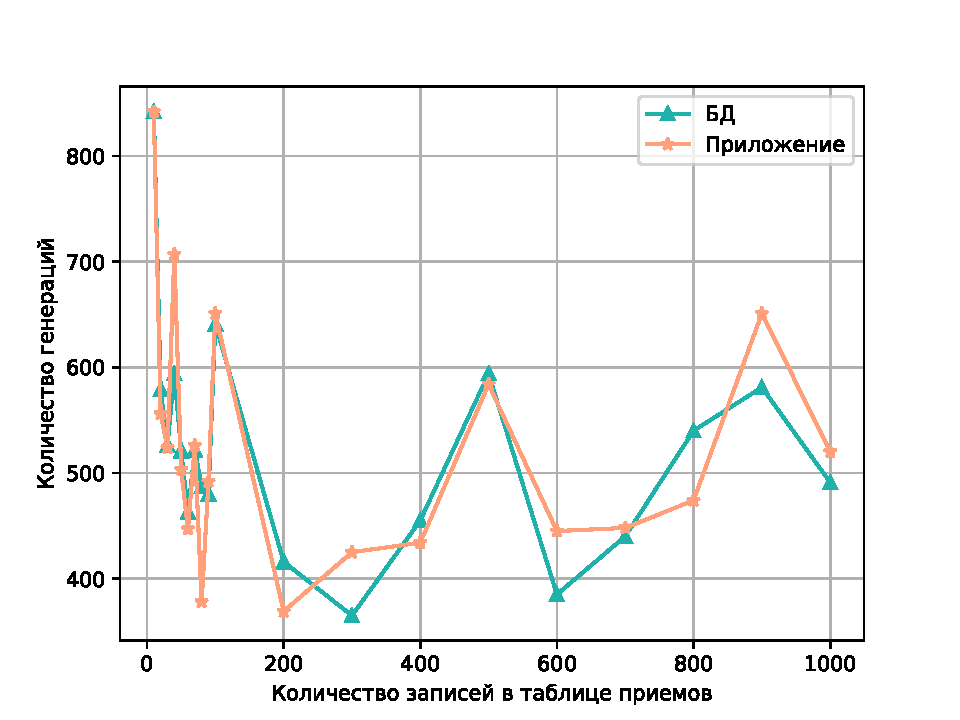
\includegraphics[width=160mm]{image/errors}
	\caption{Зависимость количества перегенераций записи на прием от размера таблицы с записями}
	\label{errors}
\end{figure}

\newpage
График зависимости времени проверки новой записи от объема данных и места, где происходят вычисления, представлен на рисунке~\ref{graph}.
\begin{figure}[!h]
	\centering
	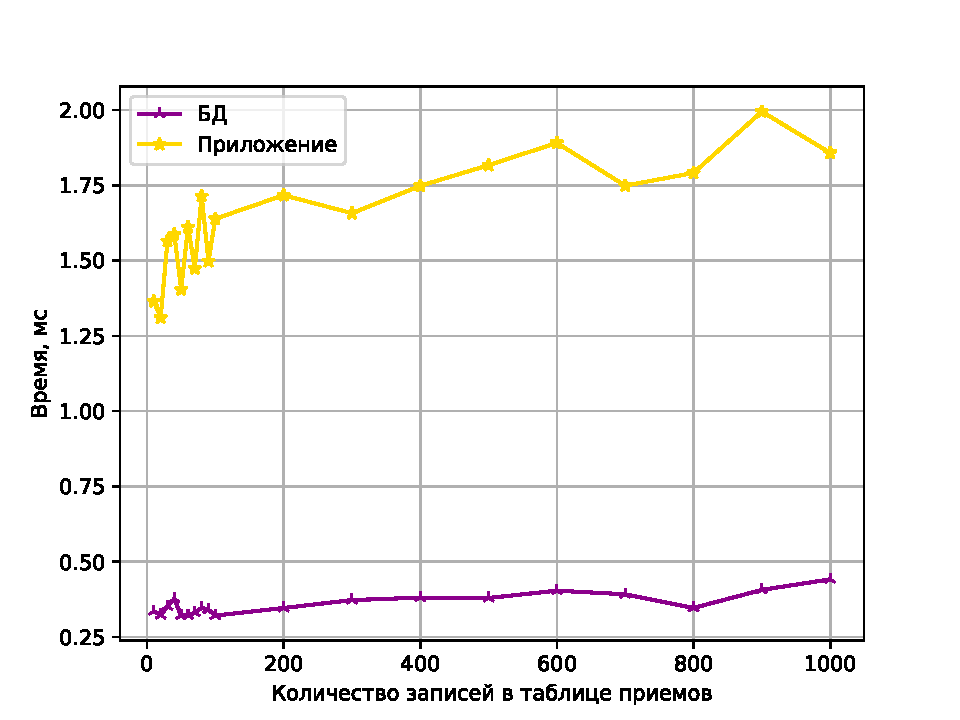
\includegraphics[width=160mm]{image/resultGraph}
	\caption{Зависимость времени проверки новой записи на прием от размера таблицы и места, где осуществляются вычисления}
	\label{graph}
\end{figure}

По результатам исследования видно, что использование триггера на уровне базы данных в среднем в 5 раз быстрее, чем использование проверок на уровне приложения. 

Также на графике присутствуют колебания до того момента, как число записей в таблице не стало больше 100. Это связано с количеством докторов, так как при таком объеме записей каждый доктор имеет 2-3 приема, а временной промежуток для них составляет год. 

Далее видно, что время для верификации новой записи на уровне приложения увеличивается быстрее, чем на уровне базы данных. Это связано с объемом передаваемой информации между приложением и базой данных, который увеличивается с каждой итерацией, так как при обработке на уровне приложения необходимо получить таблицу с записями на прием и таблицу с докторами, которая не меняется на протяжении исследования. Таким образом на уровне приложения выполняется два запроса к базе данных, что и замедляет суммарное время проверки новой записи. 


\subsection*{Вывод}
В данном разделе было описано исследование времени проверки валидности новой записи на прием от количества записей и места, где осуществляются вычисления. Исследование показало, что эффективне по времени использовать обработку записи на уровне базы данных.
